\documentclass{article}
\usepackage[utf8]{inputenc}
\usepackage{graphicx} 
\usepackage[text={18cm,21cm},centering]{geometry}

\title{Proyecto final de IA y Simulación}
\author{Juan Carlos Espinosa Delgado C-411 \\
        Raudel Gómez Molina C-411\\
        Alex Sierra Alcalá C-411
}
\date{28 de arbil de 2024}
\begin{document}

\maketitle
\newpage

\tableofcontents
\newpage

\section{Introducción}
El fútbol es un deporte de equipo muy popular en todo el mundo, y su simulación mediante técnicas de inteligencia
artificial (IA) se ha convertido en un área de investigación activa. La simulación de partidos de fútbol permite a
los investigadores y profesionales del deporte estudiar diferentes estrategias, tácticas y escenarios de juego sin la
necesidad de partidos físicos reales.

Este informe presenta los resultados de un proyecto de simulación de un partido de fútbol utilizando técnicas de IA. 
El objetivo del proyecto era desarrollar un modelo de simulación que pudiera generar partidos de fútbol realistas y 
que permitiera a los usuarios experimentar con diferentes parámetros y estrategias para hacer predicciones de estos 
partidos.
\newpage
\section{Modelación basada en Agentes}
Para realizar simulaciones de los juegos hacemos uso de agentes inteligentes, nuestro
ambiente consistirá en el estado actual del juego, que está compuesto por sus jugadores, la
estrategia que siguen, sus atributos de jugador actuales, los entrenadores, el terreno y las 
estadísticas actuales del partido.Nuestros agentes serán los jugadores y entrenadores y su función 
objetivo será ganar el partido.

\subsection{Modelación del ambiente}
Nuestro ambiente consta de las siguientes características:

\begin{enumerate}
      \item \textbf{Accesibilidad}: Nuestro ambiente es totalmente accesible, cada jugador posee conocimiento acerca del
            resto de los jugadores y de sus posiciones en el terreno, de dónde se encuentra el balón y de las estadísticas 
            actuales del partido. Importante aclarar que para los jugadores se tiene en cuenta un atributo de visión y 
            cansancio, que limita las acciones que este puede tomar.
            
      \item \textbf{Determinista o no determinista}: Nuestro ambiente es un ambiente no determinista, ya que, al no
            conocer el resultado de cada acción con certeza, existe incertidumbre acerca del estado del ambiente luego de 
            realizar una acción.
            
      \item \textbf{Episódico o secuencial}: Este ambiente es secuencial, ya que las decisiones del agente pueden
            influir de forma positiva o negativa en el futuro, por lo que tiene que razonar las consecuencias de sus acciones.
            
      \item \textbf{Estático o dinámico}: Es un ambiente estático, ya que permanece inalterable mientras no se
            realice una acción sobre él, de hecho, todos los jugadores deben realizar su acción (la cual puede ser no hacer 
            nada) para poder avanzar en el partido.
            
      \item \textbf{Discreto o continuo}: Optamos por que el tiempo fuera discreto, aunque eso no aleje un poco de la
            realidad. En cada instancia de tiempo, cada jugador puede realizar un número constante de acciones (solo una). 
            Cada jugador no puede decidir de forma independiente el instante exacto de tiempo en que realizará su acción, 
            sino que se sigue un orden preestablecido en cada instancia de tiempo. Todas estas consideraciones simplifican 
            de forma considerable el problema aunque lo alejan un poco de la realidad.
            
\end{enumerate}

\subsection{Tipos de Agentes}

\subsubsection{Agente jugador}
Nuestros jugadores son agentes puramente reactivos ya que basan su decisión enteramente en el presente, sin referencia 
a lo que haya pasado anteriormente. Estos simplemente responden directamente al ambiente. Implementamos varias 
estrategias que pueden ser usadas por el agente. Estas perfectamente pueden ser combinadas en un mismo juego por 
varios agentes y actúan de forma independiente.

Una de estas estrategias se basa en tipos de comportamiento entre los que se encuentran: ofensivo, defensivo, evitar 
cansancio y el respeto por la posición inicial impuesta por el entrenador. En dependencia de si los jugadores son 
defensas, mediocampistas o delanteros, tendrán una estrategia basada en una heurística, la cual funciona dándole 
pesos a cada uno de los comportamientos del agente, y un pequeño peso a un comportamiento aleatorio. De esta forma 
cada jugador puede variar su configuración de comportamiento en dependencia de su posición en la alineación.

Otra estrategia implementada se basa en la búsqueda del posible árbol de juego (esta implementación tuvo sus complicaciones 
ya que las transiciones de posibles acciones son no deterministas). Por esta razón 
optamos por evaluar todas las posibles acciones del agente y tomando cada una de estas simular el comportamiento del 
resto de los agentes y en la próxima instancia de tiempo volver a evaluar todas las posibles acciones del agente y así 
hasta cierto nivel que se especifica. Una vez finalizadas estas simulaciones se evalúa que tan bueno es la posición 
obtenida en el campo usando una función de evaluación y se toma la mejor decisión en base a este número. En esta 
función se le da una valoración a qué tan bien está posicionado el equipo del jugador ofensivamente en caso de tener 
el balón o defensivamente en caso de que la posesión sea del equipo contrario. Para hacer esta valoración tenemos en 
cuenta la posición del balón y la distancia a la que este se encuentra de la portería rival, las oportunidades de 
pase, el marcador actual del partido y se hace una valoración también de la ventaja que tiene un equipo sobre otro 
en el terreno haciendo uso de las estadísticas del partido con diferentes pesos en donde por ejemplo se usan los 
goles, faltas, pases, pases, tiros y tarjetas, donde un gol tiene bastante mas peso que un pase  o un disparo. 
Teniendo en cuenta los valores numéricos todos estos factores el jugador evalúa la posición ofensiva/defensiva de 
su equipo basado en reglas de lógica difusa donde por ejemplo, si el jugador considera que un atacante está lejos 
(según lo que considere lejos ese jugador) de la portería rival, este no tiene una posición ofensiva buena.
Todas las reglas mencionadas anteriormente se aplican al algoritmo de evaluación usando lógica difusa.


Como en la vida real, un jugador no sabe cómo percibe el resto de los jugadores los datos de un partido, este no 
tiene conocimiento de sus funciones de evaluación en nuestra simulación, por lo que a la hora de ejecutar la búsqueda
su predicción del partido no es del todo exacta, haciendo su pensamiento más realista. Para intuir las acciones del 
resto de los jugadores, hace uso de las heurísticas explicadas anteriormente, dependiendo si el jugador a predecir 
es defensor, centrocampista o delantero, teniendo en cuenta los comportamientos más probables de estos tipos de 
jugadores.

\subsubsection{Agente entrenador}
Nuestros agentes entrenadores, son agentes puramente reactivos ya que, al igual que los jugadores, basan 
su decisión enteramente en el presente, sin referencia a lo que haya pasado anteriormente.

Su primera tarea será la de elegir el 11 inicial. Para ello tienen distintas posibilidades de formaciones 
(4-3-3, 5-3-2, etc). Para cada formación eligen a los 11 jugadores haciendo uso de una heurística que consiste en 
que el mejor 11 posible a alinear es aquel que mejores jugadores tenga en general (basado en los atributos de los 
jugadores de nuestro dataset). Optamos por este heurística de evaluación un tanto greedy ya que evaluar todas las 
combinaciones sobre el campo de los jugadores es un problema combinatorio muy costoso computacionalmente, esto tiene la
desventaja que solo se evalúa el jugador que mejor para una posición y no existe una evaluación conjunta. El entrenador 
explora todas las combinaciones de 11 jugadores posibles de la plantilla en donde ningún jugador esté fuera de 
posición (por ejemplo no ve ninguna combinación en la que Messi sea portero) todo esto después de aplicar la 
heurística descrita anteriormente. Luego de elegir para cada formación su mejor alineación, el entrenador simula 
varias veces todas sus formaciones posibles y las del entrenador rival y decide alinear la que màs porcentaje de 
victoria le dé. Al ser no determinista nuestra simulación y no saber el resultado de cada acción en el juego con 
certeza, no pudimos hacer usos de algoritmos como el \textbf{MTCS} para el cual está probada su eficacia en este tipo de 
contextos pero en el caso de los deterministas, por lo que se optó por la idea descrita anteriormente.

Una vez empezado el partido con las alineaciones decididas por cada entrenador, estos también pueden ejecutar 
acciones. Entre estas se encuentran hacer cambios de jugadores y cambios de formaciones. En los cambios de 
formaciones los entrenadores si podrán situar jugadores en posiciones que no aparezcan entre las posibles a jugar 
por estos, teniendo una penalización en sus atributos de habilidades (ya que en la vida real los jugadores que juegan 
fuera de sus posiciones habituales no son igual de buenos que en estas). Para tomar las decisiones sobre qué acción 
ejecutar, los entrenadores siguen el mismo algoritmo descrito para elegir la alineación inicial pero en este caso 
asumen que el técnico rival jugará random ya que no es posible probar todas las posibles acciones y llegar hasta el 
final del partido.

Otra estrategia implementada para los entrenadores es siguiendo la misma idea que la búsqueda de los jugadores.
En este caso es mucho más fácil ya que solo se tiene en cuenta la interacción de los dos entrenadores, por lo que en este
caso se puede hacer uso de una especie de \textbf{minimax} (con el no determinismo de las transiciones presente). Para la ejecución del mismo
se evalúan todas las posibles acciones de ambos entrenadores y se simula hasta la próxima instancia de tiempo en que le corresponda
jugar, así hasta llegar a bajar una cantidad de niveles y luego utilizar la misma evaluación del campo que utilizaban los jugadores
más simplificada.   

\subsection{Características de los agentes}

\begin{enumerate}
      \item \textbf{Reactivos}: Estos agentes toman decisiones basadas únicamente en la información inmediata del entorno. Responden 
      directamente a estímulos o cambios en el entorno. En el contexto de nuestra simulación, los agentes jugadores reaccionan instantáneamente 
      a la posición y movimiento del balón, tomando deciciones en todo momento para lograr sus objetivos.

      \item \textbf{Proactivos}: Estos agentes planifican y anticipan posibles escenarios futuros en lugar de simplemente reaccionar a 
      eventos actuales. Estos agentes pueden tomar decisiones considerando un objetivo a largo plazo y diseñando estrategias para alcanzarlo. 
      En nuestro proyecto, los entrenadores podrían actuar como agentes proactivos al planificar la alineación del equipo, realizar cambios 
      tácticos durante el partido y ajustar la estrategia en función del desarrollo del juego.

\end{enumerate}

\section{Simulación de partidos}

\subsection{Campo de juego y posiciones}

El terreno de juego se representa gráficamente con un
array de 20 filas por 11 columnas donde se intenta simular un campo de fútbol real, con límites por los lados y por 
el fondo, y con dos porterías. Una vez que introducimos a los jugadores en el campo para simular un partido, ocupan 
las posiciones predeterminadas para cada posición, que varían dependiendo de la táctica utilizada. Aquí podemos ver 
un ejemplo de las formaciones iniciales de un partido y de las posiciones que existen: 

\includegraphics*[width=0.9\textwidth]{filed.jpg}
\bigskip

\includegraphics*[width=0.9\textwidth]{report_table.jpg}
\bigskip


\subsection{Atributos de los jugadores}
Los datos de los equipos y jugadores son extraídos de un dataset del FIFA 22 de EA Sports. Un jugador tiene un nombre, 
un conjunto de posiciones, equipo al que pertenece, un dorsal y, además, doce atributos preestablecidos. A 
continuación una relación de en què acciones se usa cada uno de los atributos:

\includegraphics*[width=0.9\textwidth]{attributed_table.jpg}
\bigskip

Además de los atributos vistos en la tabla anterior, hacemos uso de la resistencia de los jugadores. cada acción que realiza un jugador tiene un costo de estamina. Existe también la acción de moverse en  el terreno, tanto con balón como sin él, donde lo único que sucede es la disminución de estamina sin tener que utilizar ninguno de los atributos de la tabla.

Los atributos preestablecidos son valores numéricos previamente asignados en el dataset, con valores posibles del 1 al 
99, pero que generalmente se encuentran entre 60 y 85, donde se evalúa de forma precisa cómo de bueno es un jugador en 
un aspecto físico o técnico a la hora de jugar un partido. Para poner un ejemplo, un atributo es la Velocidad. Si un 
jugador llamado JUGADOR1 tiene un valor de 83 de velocidad, y otro jugador llamado JUGADOR2 tiene un valor de 70 de 
velocidad, significa que el JUGADOR1 es más rápido que el JUGADOR2. Esto quiere decir que, a la hora de jugar el 
partido, es más probable que JUGADOR1 gane a JUGADOR2 en velocidad. Es importante no confundir esta última frase. 
Es más probable que JUGADOR1 gane a JUGADOR2 en velocidad, pero no significa que JUGADOR1 gane a JUGADOR2 siempre.

Para explicar cuál es la probabilidad de que gane uno u otro jugador,
explicaremos a continuación cómo funciona el algoritmo de probabilidades:

Supongamos que ocurre un pase, donde el receptor (del equipo atacante) tiene 81 en reacciones y 85 en control del 
balón y el defensa que quiere interceptar tiene 68 en intercepción y 72 en defensa. Hacemos una normalización que 
no es màs que la media de los atributos implicados del jugador y sacaremos un valor aleatorio entre ese factor y 99. 
Ese será nuestro factor de aleatoriedad.


\includegraphics*[width=0.9\textwidth]{rank.jpg}
\bigskip

Con estos datos, podemos afirmar que, si JUGADOR1 y JUGADOR2 disputasen una recepción de un pase en medio de un 
partido, JUGADOR1 tendría más posibilidades de ganarla, pero esto no implica que tenga que ganar siempre.
Obviamente, cuanta más diferencia hay entre los valores de los jugadores, más fácil es ganar el algoritmo de 
aleatoriedad para el de valor superior. En caso de empate en los factores de aleatoriedad ganará el duelo el 
jugador a la defensa.

\subsection{Acciones de los jugadores}

Como ya mencionamos anteriormente las acciones de los jugadores ocurren en una instancia de tiempo en la que cada agente decide 
una única acción para realizar. El orden en que los agentes deciden sus acciones es secuencial y se basa en la posición que estos tengan en el campo,
comenzando por el jugador que tiene la pelota. Las acciones que pueden realizar los jugadores son las siguientes:

\begin{enumerate}
      \item \textbf{Nothing}: El jugador entre sus decisiones posibles tiene la de no hacer nada, esta es la única que no resta estamina.
            
      \item \textbf{Pass}: El jugador con balón tiene la posibilidad de pasar la pelota a los compañeros que se encuentre en su rango de vision, el pase siempre llega con éxito.
            
      \item \textbf{Move}: Todo jugador tiene la posibilidad de moverse sobre el terreno, la única limitante es que no se puede mover a un lugar donde ya haya un jugador.
            
      \item \textbf{Dribble}: Junto con la acción de moverse con el balón, el jugador puede decidir si intentar regatear para que los defensores de las casillas contiguas a la casilla objetivo no le roben el balón.
            
      \item \textbf{StealBall}: Los jugadores a la defensa tienen la posibilidad de robar el balón si alguien del equipo rival recibe un pase  o se mueve con el balón hacia una casilla contigua a la suya.
            
      \item \textbf{Shoot}: Los jugadores con balón siempre tienen la oportunidad de disparar, con un probabilidad de que el balón vaya a portería en dependencia de su habilidad de tiro y distancia a esta, y en caso de que vaya a puerta hay otra probabilidad de que sea gol.
            
\end{enumerate}


\subsection{Acciones de los entrenadores}

Los entrenadores no pueden actuar en todas las instancias de tiempo al igual que los jugadores esto tratando de imitar la realidad
en la que en todo momento los entrenadores no realizan sus acciones. Las acciones que ejecuten los entrenadores solo
serán aplicadas una vez que se reorganice el juego en el campo, esto solo ocurre cuando se produce un disparo a portería.
Las posibles acciones de los entrenadores son las siguientes:

\begin{enumerate}
      \item \textbf{entrenadorNothing}: El entrenador entre sus decisiones posibles tiene la de no hacer nada.
            
      \item \textbf{ChangePlayer}: El entrenador tiene la posibilidad de cambiar jugadores del terreno por otros que pertenezcan a su lista de jugadores posibles a alinear siempre que le queden cambios.
            
      \item \textbf{ChangeLineUp}: Todo entrenador tiene la posibilidad de cambiar la formación en medio de un partido, penalizando a los jugadores que queden jugando fuera de sus posiciones habituales.
            
\end{enumerate}


\section{Integración con LLM}

El componente de \textbf{NLP} que usamos en nuestro proyecto fue darle la facilidad al usuario que desea realizar la simulación del 
juego de fútbol la posibilidad de configurar dicha simulación en lenguaje natural. Para completar esta tarea usamos la api de \textbf{Gemini}
en su versión pro, la idea básica fue realizar trabajo de \textbf{prompt engineer} a la consulta realizada por el usuario y así obtener
la consulta original en un formato que se acople a nuestro sistema.

Los posibles parámetros de configuración de la simulación son los siguientes:

\begin{itemize}
      \item \textbf{Equipos implicados en la simulación}: para obtener estos parámetros optamos por filtrar primero los
            equipos por liga ya que era imposible proporcionarle al modelo todos los equipos de nuestro dataset, así que primero
            el usuario deberá especificar la liga y luego los equipos implicados en el juego. Por tanto primero se le pide al
            modelo que identifique de todas las posibles ligas la que especificó el usuario y luego se le proporcionan todos
            los equipos de dicha liga y se le pide seleccionar el equipo local y el equipo visitante en el siguiente formato:
            FC Barcelona vs CF Real Madrid.
            
      \item \textbf{Estrategia de los entrenadores para elegir la alineación}: las posibles estrategias para el entrenador en este
            caso son \textbf{random} y \textbf{simulate} las cuales están basadas en las estrategias descritas anteriormente. Por lo
            que entonces se le pide al modelo que identifique estos parámetros.
            
      \item \textbf{Estrategia de los entrenadores para elegir las acciones durante el juego}: las posibles estrategias para el entrenador en este
            caso son \textbf{random}, \textbf{simulate} y \textbf{minimax} las cuales están basadas en las estrategias descritas anteriormente. Por lo
            que entonces se le pide al modelo que identifique estos parámetros.
            
      \item \textbf{Estrategia de los jugadores para elegir las acciones durante el juego}: las posibles estrategias para los jugadores en este
            caso son \textbf{random}, \textbf{heuristic} y \textbf{minimax} las cuales están basadas en las estrategias descritas anteriormente. Por lo
            que entonces se le pide al modelo que identifique estos parámetros.
            
            
\end{itemize}

\includegraphics*[width=0.9\textwidth]{llm.png}
\bigskip

\section{Detalles de implementación}

\subsection{Mecanismo de simulación}

Como estamos haciendo uso de varios algoritmos de búsqueda para la ejecución de las acciones de los agentes durante el juego
fue necesario la creación de un mecanismo de memoria sobre las acciones que se ejecutan. Para ello se encapsuló la lógica de cada 
acción en la clase \textbf{Action} a la cual se le implementaron las funciones \textbf{execute} y \textbf{reset}. Siguiendo esta idea se definió
un mecanismo de \textbf{Dispatch} mediante le cual los agentes ejecutan sus acciones y estas se guardan en un pila (\textbf{stack}) para después poder 
ser reseteadas en el momento que así se requiera. En el caso de las acciones de los entrenadors que no tiene un efecto inmediato se hace 
uso de una nueva pila (\textbf{lazy\_stack}) en la cual se introducen estas acciones y en el momento indicado se comprimen y se aplican
al juego de manera análoga a lo anterior este mecanismo de acciones lazy también cuenta con un mecanismo de \textbf{reset}.

Para simular el juego en concreto de hace uso de una clase \textbf{Simulator} la cual se encarga de ejecutar una instancia de tiempo
y resetear una instancia de tiempo.

Para proveer un mecanismo de simulación de los agentes se emplea la clase \textbf{SimulatorAgent} la cual posee una función para simular 
el resto del comportamiento del medio que así lo requiera el agente, una función para simular el resto de la instancia de tiempo correspondiente
así como las respectivas funciones de reset de cada una de las funciones antes mencionadas. Además se le provee al agente una función para interactuar
directamente con el \textbf{Dispatch} del juego.

\subsection{Implementación de reglas y lógica difusa}

Usamos un sistema de lógica difusa para determinar qué tan buenas eran las posiciones defensivas y ofensivas de los jugadores 
sobre el terreno en un partido de fútbol. El sistema consta de dos partes principales: una para determinar las posiciones 
defensivas y otra para las posiciones ofensivas. Cada parte utiliza variables de entrada y salida difusas, así como reglas 
difusas para mapear las entradas a las salidas correspondientes.

Ambas tienen las mismas variables de entrada:
\begin{itemize}
      \item Distancia a la posición inicial en el Line-Up (baja, media, alta).
            
      \item Distancia al balón (baja, media, alta).
            
      \item Función del jugador (defensa, centrocampista o delantero).
\end{itemize}

Mientras que las variables de salida son:
\begin{itemize}
      \item Posicionamiento defensivo.
            
      \item Posicionamiento ofensivo.
\end{itemize}


Cada una con posibles valores de bueno, normal y malo en el conjunto difuso al que pertenecen.

Para su implementación se utilizó la biblioteca scikit-fuzzy de Python. Se han definido antecedentes y consecuentes difusos, 
así como reglas difusas para cada parte del sistema. 

Los valores obtenidos usando estas funciones, se promedian para todos los jugadores de un mismo equipo, para tener una idea de 
qué tan bien parados están de forma conjunta sobre el terreno. Esta es una de las métricas usadas para desarrollar la función de 
evaluacion sobre una instancia del juego.

El sistema de lógica difusa proporciona una forma flexible y adaptable de determinar el valor de las posiciones de los jugadores 
en un partido de fútbol. Al considerar múltiples variables y reglas difusas, el sistema puede tomar decisiones inteligentes en 
tiempo real para optimizar el rendimiento defensivo y ofensivo del equipo.

\subsection{Encapsulamiento de las estrategias de los agentes}

Para cada tipo de acción de los agentes (jugar para los jugadores, realizar acciones durante el partido y establecer alineación para los
técnicos) se crea una interfaz que permite encapsular dicho comportamiento y que sea posible permitir más de una configuración sin afectar
el resto del funcionamiento del agente.

\section{Análisis experimental}

Con el objetivo de evaluar el rendimiento de nuestro sistema de simulación, realizamos una serie de experimentos para medir
la eficacia de las diferentes estrategias de los agentes y la influencia de los parámetros de configuración en el resultado.
Para ello, simulamos varios partidos de fútbol con diferentes configuraciones heurísticas vs configuraciones 
aleatorias y analizamos los resultados obtenidos en cuanto a las estadísticas de los jugadores.

\subsection{Experimento 1: Comparación de estrategias de selección de acciones de los jugadores}
Agente Jugador inteligente:

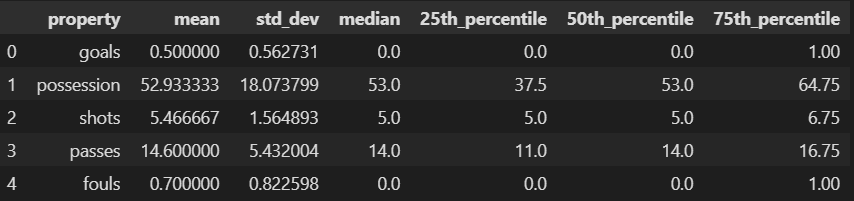
\includegraphics[width=0.9\textwidth]{tabla1.PNG}

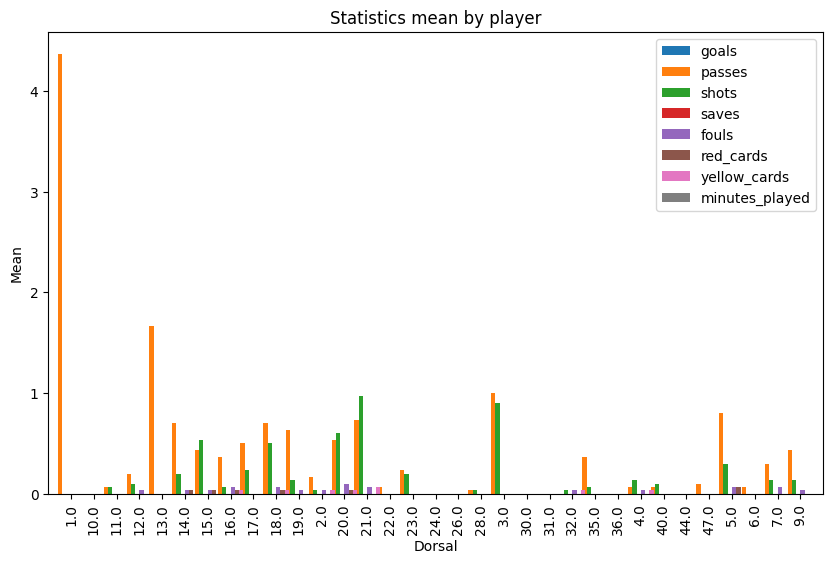
\includegraphics[width=0.9\textwidth,height=0.5\textwidth]{smart_vs_random_player_home.png}

Agente Jugador aleatorio:

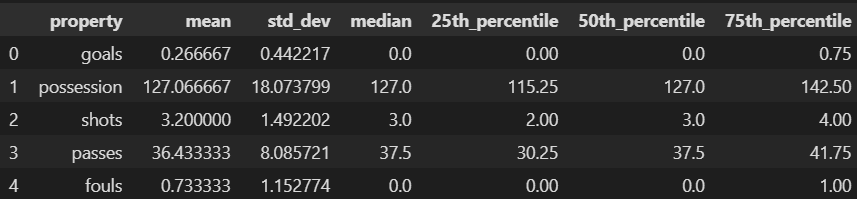
\includegraphics[width=0.9\textwidth]{tabla2.PNG}

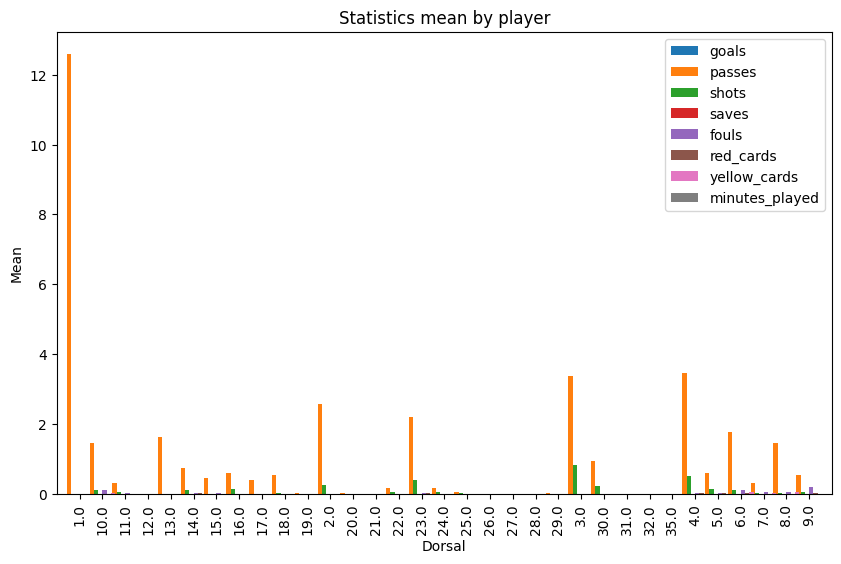
\includegraphics[width=0.9\textwidth,height=0.5\textwidth]{smart_vs_random_player_away.png}                       

\subsection{Experimento 2: Comparación de estrategias de selección de alineación de los entrenadores}
Agente Entrenador inteligente:

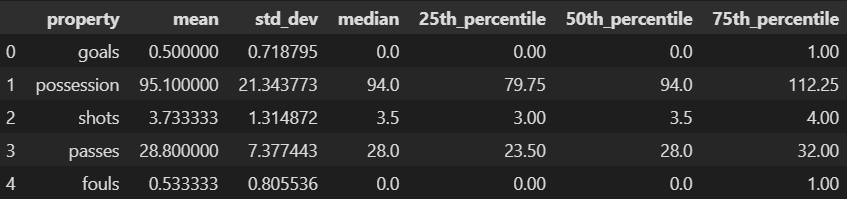
\includegraphics[width=0.9\textwidth]{tabla3.PNG}

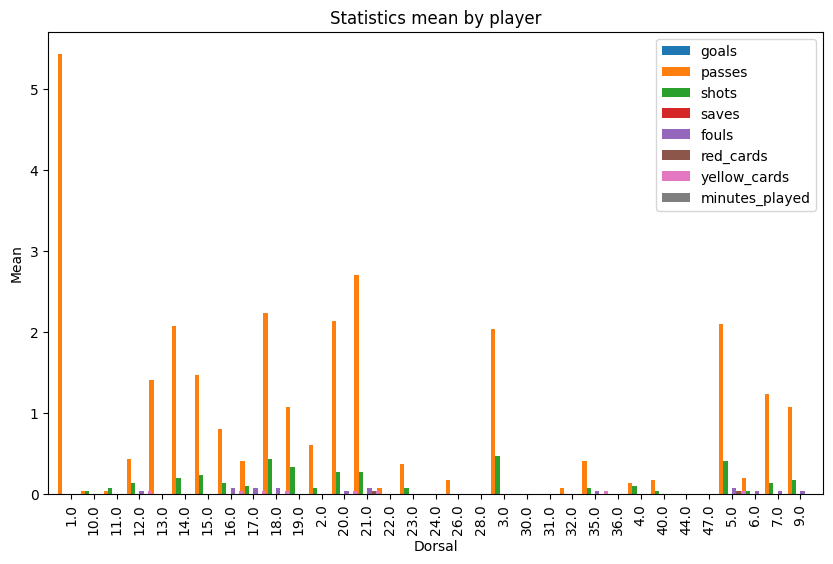
\includegraphics[width=0.9\textwidth,height=0.5\textwidth]{smart_vs_random_line_up_home.png}

Agente Entrenador aleatorio:

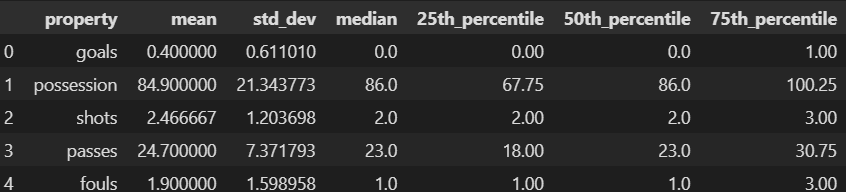
\includegraphics[width=0.9\textwidth]{tabla4.PNG}

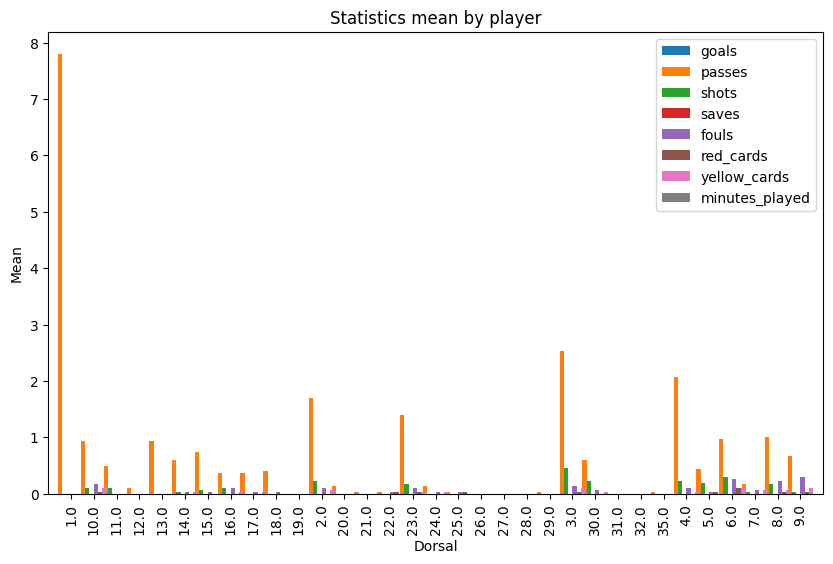
\includegraphics[width=0.9\textwidth,height=0.5\textwidth]{smart_vs_random_line_up_away.png}                       

\subsection{Experimento 3: Comparación de estrategias de selección de acciones de los entrenadores}
Agente Entrenador minimax:

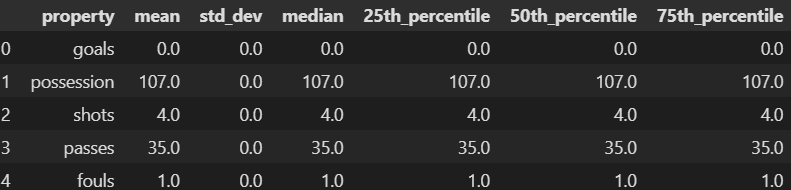
\includegraphics[width=0.9\textwidth]{tabla5.PNG}

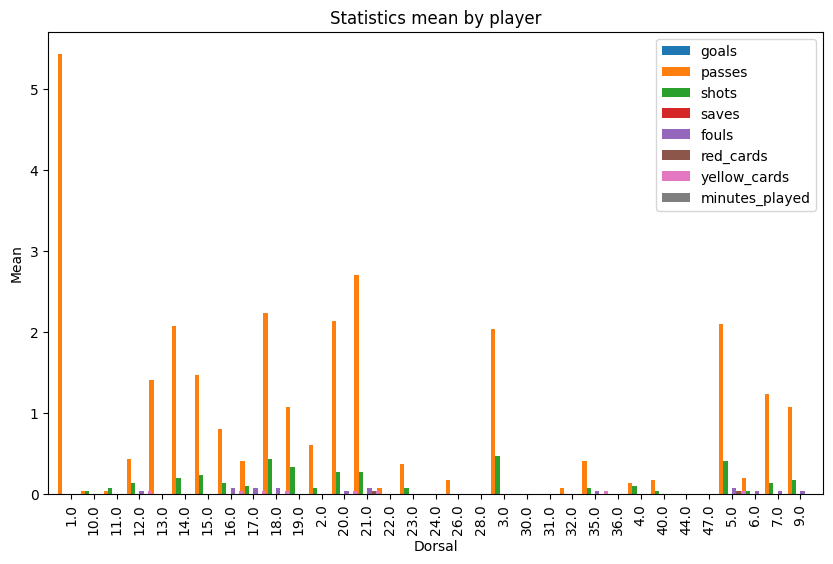
\includegraphics[width=0.9\textwidth,height=0.5\textwidth]{smart_vs_random_line_up_home.png}

Agente Entrenador aleatorio:

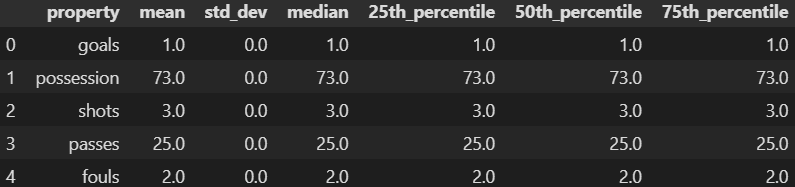
\includegraphics[width=0.9\textwidth]{tabla6.PNG}

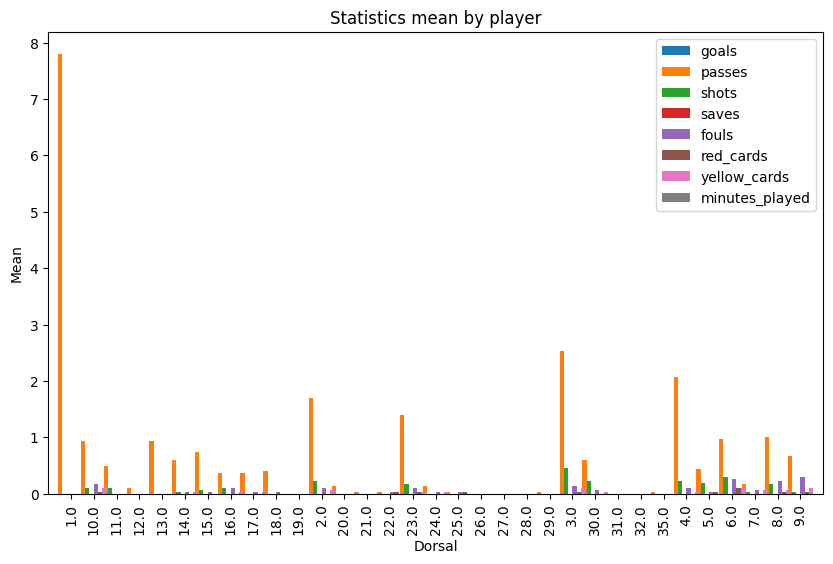
\includegraphics[width=0.9\textwidth,height=0.5\textwidth]{smart_vs_random_line_up_away.png}

\subsection{Datos generales}

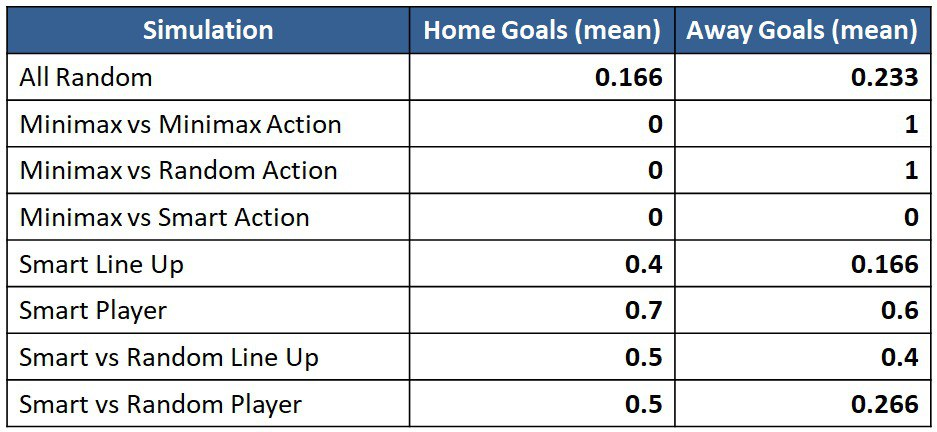
\includegraphics[width=0.9\textwidth]{general_data.jpg}

\subsection{Análisis de los resultados}
Los resultados de los experimentos muestran que las estrategias de selección de acciones de los jugadores y selección de acciones y alineación de los entrenadores
tienen un ligero impacto en el rendimiento de las estadísticas de los jugadores, y por tanto, de los equipos en un partido de fútbol. En general, los agentes inteligentes
tuvieron un mejor desempeño que los agentes aleatorios, lo que sugiere que nuestras implementaciones basadas en heurísticas y algoritmos de búsqueda son efectivas para
mejorar el rendimiento de los agentes en un partido de fútbol. Sin embargo, las diferencias no son tan representativas como esperábamos.

El resto de los experimentos incluyendo tablas de resultados y gráficos se encuentran en el repositorio del proyecto en el archivo \texttt{src/data\_analysis.ipynb}.

\section{Conclusiones}

En este trabajo, aplicamos nuestros conocimientos en inteligencia artificial (IA) y simulación para analizar algunas estrategias, tanto de entrenadores como de jugadores en un partido de fútbol.
Nuestro sistema de simulación de partidos de fútbol basado en agentes inteligentes es capaz de generar partidos realistas y permitir a los usuarios experimentar con diferentes parámetros y estrategias para hacer predicciones de estos partidos.
Aunque no logramos identificar una estrategia del todo buena de manera general,
encontramos que ciertas estrategias son algo efectivas en escenarios específicos como en la elección de la alineación de los entrenadores y en la selección de acciones de los jugadores.
Si bien los resultados obtenidos muestran un rendimiento no tan bueno de estas estrategias, creemos que con más tiempo y recursos podríamos mejorar el rendimiento de los agentes,
sobre todo mediante el refinamiento de las heurísticas de evaluación y la exploración de estrategias de búsqueda más avanzadas. Además, este trabajo ha destacado la importancia de investigar más a fondo la interacción entre diferentes agentes en un entorno colaborativo y no determinista como es un partido de fútbol.
En general, nuestra conclusión del proyecto es que los resultados no son del todo satisfactorios teniendo en cuenta las espectativas iniciales, 
destacando la complejidad inherente de modelar y predecir el comportamiento en un entorno tan dinámico como un partido de fútbol, donde intervienen numerosas variables y factores impredecibles.
En última instancia, este proyecto sienta las bases para futuras investigaciones en el campo de la inteligencia artificial aplicada al fútbol. La experiencia adquirida y los resultados obtenidos proporcionan una base para continuar explorando y mejorando las estrategias de juego, con el objetivo final de crear sistemas más sofisticados y efectivos para la simulación y análisis de partidos de fútbol.


\section{Recomendaciones}

% Para futuros trabajos se recomienda un estudio más profundo del problema que permita el desarrollo de mejores heurísticas de evaluación
% que las planteadas en este trabajo. Por ejemplo no nos fue posible desarrollar una buena heurística para las acciones del entrenador y algunas
% de las introducidas para escoger la alineación o escoger el mejor cambio las consideramos que no evalúan la alineación en conjunto.
% Además de consideramos importante mejorar las heurísticas empleadas en la función de evaluación lo que permitirá un mejor rendimiento 
% de los algoritmos de búsqueda. Otra idea no abordada en este trabajo pudiera consistir en la planificación de acciones conjuntas y 
% colaborativas para la realización de acciones en equipo.

% El estudio de mejores estrategias de búsqueda para este tipo de escenarios que pueden llegar a ser colaborativos y no deterministas puede
% ser otro punto importante para mejoras futuras.

% Otro aspecto que queremos resaltar y no exploramos del todo es el reajuste de los pesos con que cuentan las estrategias heurísticas de los jugadores
% que en futuras implementaciones se pudiera tratar de desarrollar un algoritmo que sea capaz de reajustar estos parámetros en base a la experiencia
% obtenida por el agente.

Para futuras investigaciones, se recomienda realizar un análisis más exhaustivo del problema con el fin de desarrollar heurísticas de evaluación más 
efectivas que las propuestas en este trabajo. Por ejemplo, encontramos desafíos al intentar diseñar una heurística adecuada para las decisiones del entrenador, 
así como algunas limitaciones en las estrategias introducidas para la selección de alineaciones y cambios, ya que no consideran de manera integral la 
dinámica del equipo. Asimismo, consideramos crucial mejorar las heurísticas utilizadas en la función de evaluación de una instancia del terreno, lo que 
potenciará el rendimiento de los algoritmos de búsqueda.

Una idea no explorada en este trabajo es el uso de prácticas de inteligencia artificial para la planificación de acciones colaborativas y coordinadas 
con el objetivo ejecutar acciones en equipo, lo que podría ser un enfoque prometedor. Además, el estudio de estrategias de búsqueda más efectivas en 
escenarios colaborativos y no deterministas representa otro aspecto importante para futuras mejoras.

También es relevante destacar que no abordamos completamente un ajusye inteligente de los pesos asociados a las estrategias heurísticas de los jugadores. 
En futuras implementaciones, sería interesante explorar algoritmos capaces de reajustar estos parámetros en función de la experiencia adquirida por el 
agente durante el juego, lo que podría mejorar significativamente su desempeño en situaciones variables y cambiantes.


\end{document}
